\documentclass{beamer}
\usetheme{Madrid}

\usepackage{textpos}
\usepackage{tikz}
\usetikzlibrary{calc}
%% Colors
\def \BLUE {blue}
\def \GREEN {green}
\def \ORANGE {orange}
\def \RED {red}
\def \VIOLET {violet}
\def \YELLOW {lime}

    % This file is part of nrf_seminar.

    % nrf_seminar is free software: you can redistribute it and/or modify
    % it under the terms of the GNU General Public License as published by
    % the Free Software Foundation, either version 3 of the License, or
    % (at your option) any later version.

    % nrf_seminar is distributed in the hope that it will be useful,
    % but WITHOUT ANY WARRANTY; without even the implied warranty of
    % MERCHANTABILITY or FITNESS FOR A PARTICULAR PURPOSE.  See the
    % GNU General Public License for more details.

    % You should have received a copy of the GNU General Public License
    % along with nrf_seminar.  If not, see <https://www.gnu.org/licenses/>.

\makeatletter
\setbeamertemplate{footline}
{
  \leavevmode
  \hbox{%
  \begin{beamercolorbox}[wd=.20\paperwidth,ht=2.25ex,dp=1ex,center]{author in head/foot}%
    \usebeamerfont{author in head/foot}\insertshortauthor
  \end{beamercolorbox}%
  \begin{beamercolorbox}[wd=.30\paperwidth,ht=2.25ex,dp=1ex,center]{title in head/foot}%
    \usebeamerfont{title in head/foot}\insertshorttitle
  \end{beamercolorbox}%
  \begin{beamercolorbox}[wd=.25\paperwidth,ht=2.25ex,dp=1ex,center]{author in head/foot}%
    \usebeamerfont{author in head/foot}{Advances in Physics Seminar}
  \end{beamercolorbox}%
  \begin{beamercolorbox}[wd=.25\paperwidth,ht=2.25ex,dp=1ex,right]{date in head/foot}%
    \usebeamerfont{date in head/foot}\insertdate{}\hspace*{2em}
    \insertframenumber{} / \inserttotalframenumber\hspace*{2ex} 
  \end{beamercolorbox}}%
  \vskip0pt%
}
\makeatother

\title{Nuclear Resonance Fluorescence}
\subtitle{Renaissance of a 70-year-old Techique}
\author[U. Friman-Gayer]{Udo Friman-Gayer\inst{1,2}}
\institute{
    \inst{1} Department of Physics and Astronomy, University of North Carolina at Chapel Hill, Chapel Hill, NC \\
    \inst{2} Triangle Universities Nuclear Laboratory, Duke University, Durham, NC
}
\date{Advances in Physics Seminar, 06/18/2020}

\begin{document}

\begin{frame}
    \titlepage
\end{frame}

\begin{frame}
    \frametitle{Outline}
    \tableofcontents
\end{frame}

\section{Introduction}

\subsection{'Scattering' of Photons}

\begin{frame}
    \frametitle{Interaction of Photons with Matter}
    %\def \SLIDEINRED {2}
\def \SLIDEOUTRED {3}
\def \SLIDERED {4}
\def \SLIDEGREEN {5}
\def \SLIDEBLUE {6}
\def \SLIDEVIOLET {7}

\begin{textblock}{15.}(0., -5.)
    \begin{tikzpicture}
        %%% Definitions
        %% Mathematical constants
        \def \INVERSESQRTTWO {0.7071067811865475}
        \def \NWAVEFORMSAMPLES {400}

        %% Colors
        \def \BLUE {blue}
        \def \GREEN {green}
        \def \VIOLET {violet}
        \def \RED {red}

        %% Labels
        \def \LABELLOWSTART {-1.}
        \def \LABELLOWSTOP {-2.}
        \def \LABELUPSTART {-1.}
        \def \LABELUPSTOP {-1.5}

        %% Schematic model of the nucleus
        \coordinate (NUCLEUSPOSITION) at (6., 0.);

        \def \NUCLEONRADIUS {0.3}
        \def \NUCLEONDISTANCE {1.2}
        \def \SPRINGRADIUS {0.12}

        %% Incoming EM wave
        \def \INREDAMPLITUDE {0.6}
        \def \INREDWAVEFORMLENGTH {5.}
        \def \INREDWAVELENGTH {4.}
        \def \INREDWAVESTART {0.}

        \def \INGREENAMPLITUDE {0.6}
        \def \INGREENWAVEFORMLENGTH {5.}
        \def \INGREENWAVELENGTH {1.8}
        \def \INGREENWAVESTART {0.}

        \def \INBLUEAMPLITUDE {0.6}
        \def \INBLUEWAVEFORMLENGTH {5.}
        \def \INBLUEWAVELENGTH {0.6}
        \def \INBLUEWAVESTART {0.}

        \def \INVIOLETAMPLITUDE {0.6}
        \def \INVIOLETWAVEFORMLENGTH {5.}
        \def \INVIOLETWAVELENGTH {0.3}
        \def \INVIOLETWAVESTART {0.}

        %% Outgoing EM wave(s)
        \def \OUTREDHORAMPLITUDE {0.2}
        \def \OUTREDHORWAVEFORMLENGTH {3.}
        \def \OUTREDHORWAVELENGTH {\INREDWAVELENGTH}
        \def \OUTREDHORWAVESTART {7.}

        \def \OUTREDMIDAMPLITUDE {0.2}
        \def \OUTREDMIDWAVEFORMLENGTH {3.}
        \def \OUTREDMIDWAVELENGTH {\INREDWAVELENGTH}
        \def \OUTREDMIDWAVESTART {7.}

        \def \OUTREDVERAMPLITUDE {0.2}
        \def \OUTREDVERWAVEFORMLENGTH {3.}
        \def \OUTREDVERWAVELENGTH {\INREDWAVELENGTH}
        \def \OUTREDVERWAVESTART {7.}

        \def \OUTGREENHORAMPLITUDE {0.5}
        \def \OUTGREENHORWAVEFORMLENGTH {3.}
        \def \OUTGREENHORWAVELENGTH {\INGREENWAVELENGTH}
        \def \OUTGREENHORWAVESTART {7.}

        \def \OUTGREENMIDAMPLITUDE {0.}
        \def \OUTGREENMIDWAVEFORMLENGTH {3.}
        \def \OUTGREENMIDWAVELENGTH {\INGREENWAVELENGTH}
        \def \OUTGREENMIDWAVESTART {7.}

        \def \OUTGREENVERAMPLITUDE {0.1}
        \def \OUTGREENVERWAVEFORMLENGTH {3.}
        \def \OUTGREENVERWAVELENGTH {\INGREENWAVELENGTH}
        \def \OUTGREENVERWAVESTART {7.}

        \def \OUTBLUEHORAMPLITUDE {0.5}
        \def \OUTBLUEHORWAVEFORMLENGTH {3.}
        \def \OUTBLUEHORWAVELENGTH {\INBLUEWAVELENGTH}
        \def \OUTBLUEHORWAVESTART {7.}

        \def \OUTBLUEMIDAMPLITUDE {0.}
        \def \OUTBLUEMIDWAVEFORMLENGTH {3.}
        \def \OUTBLUEMIDWAVELENGTH {\INBLUEWAVELENGTH}
        \def \OUTBLUEMIDWAVESTART {7.}

        \def \OUTBLUEVERAMPLITUDE {0.1}
        \def \OUTBLUEVERWAVEFORMLENGTH {3.}
        \def \OUTBLUEVERWAVELENGTH {\INBLUEWAVELENGTH}
        \def \OUTBLUEVERWAVESTART {7.}

        \def \OUTVIOLETHORAMPLITUDE {0.6}
        \def \OUTVIOLETHORWAVEFORMLENGTH {3.}
        \def \OUTVIOLETHORWAVELENGTH {\INVIOLETWAVELENGTH}
        \def \OUTVIOLETHORWAVESTART {7.}

        \def \OUTVIOLETMIDAMPLITUDE {0.}
        \def \OUTVIOLETMIDWAVEFORMLENGTH {3.}
        \def \OUTVIOLETMIDWAVELENGTH {\INVIOLETWAVELENGTH}
        \def \OUTVIOLETMIDWAVESTART {7.}

        \def \OUTVIOLETVERAMPLITUDE {0.}
        \def \OUTVIOLETVERWAVEFORMLENGTH {3.}
        \def \OUTVIOLETVERWAVELENGTH {\INVIOLETWAVELENGTH}
        \def \OUTVIOLETVERWAVESTART {7.}

        %%% Drawing
        %% Incoming EM wave
        \visible<\SLIDEINRED-\SLIDERED>{
            \draw [very thick, \RED, domain=\INREDWAVESTART:\INREDWAVESTART+\INREDWAVEFORMLENGTH, samples=\NWAVEFORMSAMPLES] plot (\x, {\INREDAMPLITUDE*sin(\INREDWAVEFORMLENGTH/\INREDWAVELENGTH*2*pi/4*\x r)});
        }

        \visible<\SLIDEGREEN>{
            \draw [very thick, \GREEN, domain=\INGREENWAVESTART:\INGREENWAVESTART+\INGREENWAVEFORMLENGTH, samples=\NWAVEFORMSAMPLES] plot (\x, {\INGREENAMPLITUDE*sin(\INGREENWAVEFORMLENGTH/\INGREENWAVELENGTH*2*pi/4*\x r)});
        }
        \visible<\SLIDEBLUE>{
           \draw [very thick, \BLUE, domain=\INBLUEWAVESTART:\INBLUEWAVESTART+\INBLUEWAVEFORMLENGTH, samples=\NWAVEFORMSAMPLES] plot (\x, {\INBLUEAMPLITUDE*sin(\INBLUEWAVEFORMLENGTH/\INBLUEWAVELENGTH*2*pi/4*\x r)});
        }
        \visible<\SLIDEVIOLET>{
            \draw [very thick, \VIOLET, domain=\INVIOLETWAVESTART:\INVIOLETWAVESTART+\INVIOLETWAVEFORMLENGTH, samples=\NWAVEFORMSAMPLES] plot (\x, {\INVIOLETAMPLITUDE*sin(\INVIOLETWAVEFORMLENGTH/\INVIOLETWAVELENGTH*2*pi/4*\x r)});
        }

        % Label
        \visible<\SLIDEINRED-\SLIDERED>{
            \draw [very thick, black] (\INREDWAVESTART, \LABELLOWSTART) -- (\INREDWAVESTART, \LABELLOWSTOP);
            \draw [very thick, black] (\INREDWAVESTART+\INREDWAVELENGTH, \LABELLOWSTART) -- (\INREDWAVESTART+\INREDWAVELENGTH, \LABELLOWSTOP);
            \draw [very thick, black] (\INREDWAVESTART, \LABELLOWSTOP) -- (\INREDWAVESTART + \INREDWAVELENGTH, \LABELLOWSTOP);
            \draw (\INREDWAVESTART+0.5*\INREDWAVELENGTH, \LABELLOWSTOP) node[anchor=north] {$\lambda \gg 2R$};
        }

        \visible<\SLIDEGREEN>{
            \draw [very thick, black] (\INGREENWAVESTART, \LABELLOWSTART) -- (\INGREENWAVESTART, \LABELLOWSTOP);
            \draw [very thick, black] (\INGREENWAVESTART+\INGREENWAVELENGTH, \LABELLOWSTART) -- (\INGREENWAVESTART+\INGREENWAVELENGTH, \LABELLOWSTOP);
            \draw [very thick, black] (\INGREENWAVESTART, \LABELLOWSTOP) -- (\INGREENWAVESTART + \INGREENWAVELENGTH, \LABELLOWSTOP);
            \draw (\INGREENWAVESTART+0.5*\INGREENWAVELENGTH, \LABELLOWSTOP) node[anchor=north] {$\lambda \approx 2R$};
        }

        \visible<\SLIDEBLUE>{
            \draw [very thick, black] (\INBLUEWAVESTART, \LABELLOWSTART) -- (\INBLUEWAVESTART, \LABELLOWSTOP);
            \draw [very thick, black] (\INBLUEWAVESTART+\INBLUEWAVELENGTH, \LABELLOWSTART) -- (\INBLUEWAVESTART+\INBLUEWAVELENGTH, \LABELLOWSTOP);
            \draw [very thick, black] (\INBLUEWAVESTART, \LABELLOWSTOP) -- (\INBLUEWAVESTART + \INBLUEWAVELENGTH, \LABELLOWSTOP);
            \draw (\INBLUEWAVESTART+0.5*\INBLUEWAVELENGTH, \LABELLOWSTOP) node[anchor=north] {$\lambda \approx 2r$};
        }

        \visible<\SLIDEVIOLET>{
            \draw [very thick, black] (\INVIOLETWAVESTART, \LABELLOWSTART) -- (\INVIOLETWAVESTART, \LABELLOWSTOP);
            \draw [very thick, black] (\INVIOLETWAVESTART+\INVIOLETWAVELENGTH, \LABELLOWSTART) -- (\INVIOLETWAVESTART+\INVIOLETWAVELENGTH, \LABELLOWSTOP);
            \draw [very thick, black] (\INVIOLETWAVESTART, \LABELLOWSTOP) -- (\INVIOLETWAVESTART + \INVIOLETWAVELENGTH, \LABELLOWSTOP);
            \draw (\INVIOLETWAVESTART+0.5*\INVIOLETWAVELENGTH, \LABELLOWSTOP) node[anchor=north] {$\lambda \ll 2r$};
        }

        %% Nucleus
        % Boundary
        \draw [very thick, black, dashed] (NUCLEUSPOSITION) circle [radius=\NUCLEONRADIUS+0.5*\NUCLEONDISTANCE];
        % Proton
        \draw [very thick, black, fill=black] ($ (NUCLEUSPOSITION) + 0.5*\NUCLEONDISTANCE*\INVERSESQRTTWO*(1,1) $) circle [radius = \NUCLEONRADIUS];
        % Neutron
        \draw [very thick, black, fill=white] ($ (NUCLEUSPOSITION) + 0.5*\NUCLEONDISTANCE*\INVERSESQRTTWO*(-1,-1) $) circle [radius = \NUCLEONRADIUS];

        \coordinate (COMTONUCLEONSURFACE) at ($0.5*\NUCLEONDISTANCE*\INVERSESQRTTWO*(1,1) - \NUCLEONRADIUS*\INVERSESQRTTWO*(1,1)$);

        % Spring
        \draw [very thick, black] 
        ($ (NUCLEUSPOSITION) - (COMTONUCLEONSURFACE) $)
        -- ($ (NUCLEUSPOSITION) - 0.8*(COMTONUCLEONSURFACE) + \SPRINGRADIUS*(1,-1) $)
        -- ($ (NUCLEUSPOSITION) - 0.6*(COMTONUCLEONSURFACE) + \SPRINGRADIUS*(-1,1) $)  
        -- ($ (NUCLEUSPOSITION) - 0.4*(COMTONUCLEONSURFACE) + \SPRINGRADIUS*(1,-1) $)  
        -- ($ (NUCLEUSPOSITION) - 0.2*(COMTONUCLEONSURFACE) + \SPRINGRADIUS*(-1,1) $)  
        -- ($ (NUCLEUSPOSITION)                             + \SPRINGRADIUS*(1,-1) $)  
        -- ($ (NUCLEUSPOSITION) + 0.2*(COMTONUCLEONSURFACE) + \SPRINGRADIUS*(-1,1) $)  
        -- ($ (NUCLEUSPOSITION) + 0.4*(COMTONUCLEONSURFACE) + \SPRINGRADIUS*(1,-1) $)  
        -- ($ (NUCLEUSPOSITION) + 0.6*(COMTONUCLEONSURFACE) + \SPRINGRADIUS*(-1,1) $)  
        -- ($ (NUCLEUSPOSITION) + 0.8*(COMTONUCLEONSURFACE) + \SPRINGRADIUS*(1,-1) $)   
        -- ($ (NUCLEUSPOSITION) + (COMTONUCLEONSURFACE) $);

        % Label for size of nucleus
        \draw [very thick, black] ($(NUCLEUSPOSITION) - \NUCLEONRADIUS*(1,0) -0.5*\NUCLEONDISTANCE*(1,0) + \LABELLOWSTART*(0,1) $) -- ($(NUCLEUSPOSITION) - \NUCLEONRADIUS*(1,0) - 0.5*\NUCLEONDISTANCE*(1,0) + \LABELLOWSTOP*(0,1) $);
        \draw [very thick, black] ($(NUCLEUSPOSITION) + \NUCLEONRADIUS*(1,0) + 0.5*\NUCLEONDISTANCE*(1,0) + \LABELLOWSTART*(0,1) $) -- ($(NUCLEUSPOSITION) + \NUCLEONRADIUS*(1,0) + 0.5*\NUCLEONDISTANCE*(1,0) + \LABELLOWSTOP*(0,1) $);
        \draw [very thick, black] ($(NUCLEUSPOSITION) - \NUCLEONRADIUS*(1,0) - 0.5*\NUCLEONDISTANCE*(1,0) + \LABELLOWSTOP*(0,1) $) -- ($(NUCLEUSPOSITION) + \NUCLEONRADIUS*(1,0) + 0.5*\NUCLEONDISTANCE*(1,0) + \LABELLOWSTOP*(0,1) $);
        \draw ($ (NUCLEUSPOSITION) + \LABELLOWSTOP*(0,1)$) node[anchor=north] {$2R$};

        % Label for size of nucleon
        \draw [very thick, black] ($(NUCLEUSPOSITION) - 0.5*\NUCLEONDISTANCE*\INVERSESQRTTWO*(1,0) - \NUCLEONRADIUS*(1,0) + \LABELUPSTART*(0,1)$) -- ($(NUCLEUSPOSITION) - 0.5*\NUCLEONDISTANCE*\INVERSESQRTTWO*(1,0) - \NUCLEONRADIUS*(1,0) + \LABELUPSTOP*(0,1)$);
        \draw [very thick, black] ($(NUCLEUSPOSITION) - 0.5*\NUCLEONDISTANCE*\INVERSESQRTTWO*(1,0) + \NUCLEONRADIUS*(1,0) + \LABELUPSTART*(0,1)$) -- ($(NUCLEUSPOSITION) - 0.5*\NUCLEONDISTANCE*\INVERSESQRTTWO*(1,0) + \NUCLEONRADIUS*(1,0) + \LABELUPSTOP*(0,1)$);
        \draw [very thick, black] ($(NUCLEUSPOSITION) - 0.5*\NUCLEONDISTANCE*\INVERSESQRTTWO*(1,0) - \NUCLEONRADIUS*(1,0) + \LABELUPSTOP*(0,1)$) -- ($(NUCLEUSPOSITION) - 0.5*\NUCLEONDISTANCE*\INVERSESQRTTWO*(1,0) + \NUCLEONRADIUS*(1,0) + \LABELUPSTOP*(0,1)$);
        \draw ($ (NUCLEUSPOSITION) - 0.5*\NUCLEONDISTANCE*\INVERSESQRTTWO*(1,0) + \LABELUPSTOP*(0,1) $) node[anchor=north] {$2r$};

        %% Outgoing EM wave
        \visible<\SLIDEOUTRED-\SLIDERED>{
            \draw [very thick, \RED, domain=\OUTREDHORWAVESTART:\OUTREDHORWAVESTART+\OUTREDHORWAVEFORMLENGTH, samples=\NWAVEFORMSAMPLES] plot (\x, {\OUTREDHORAMPLITUDE*sin(\INREDWAVEFORMLENGTH/\OUTREDHORWAVELENGTH*2*pi/4*\x r)});

            \draw [very thick, \RED, rotate around={35:(NUCLEUSPOSITION)}, domain=\OUTREDMIDWAVESTART:\OUTREDMIDWAVESTART+\OUTREDMIDWAVEFORMLENGTH, samples=\NWAVEFORMSAMPLES] plot (\x, {\OUTREDMIDAMPLITUDE*sin(\INREDWAVEFORMLENGTH/\OUTREDMIDWAVELENGTH*2*pi/4*\x r)});

            \draw [very thick, \RED, rotate around={70:(NUCLEUSPOSITION)}, domain=\OUTREDVERWAVESTART:\OUTREDVERWAVESTART+\OUTREDVERWAVEFORMLENGTH, samples=\NWAVEFORMSAMPLES] plot (\x, {\OUTREDVERAMPLITUDE*sin(\INREDWAVEFORMLENGTH/\OUTREDVERWAVELENGTH*2*pi/4*\x r)});
        }

        \visible<\SLIDEGREEN>{
            \draw [very thick, \GREEN, domain=\OUTGREENHORWAVESTART:\OUTGREENHORWAVESTART+\OUTGREENHORWAVEFORMLENGTH, samples=\NWAVEFORMSAMPLES] plot (\x, {\OUTGREENHORAMPLITUDE*sin(\INGREENWAVEFORMLENGTH/\OUTGREENHORWAVELENGTH*2*pi/4*\x r)});

            \draw [very thick, dashed, \GREEN, rotate around={35:(NUCLEUSPOSITION)}, domain=\OUTGREENMIDWAVESTART:\OUTGREENMIDWAVESTART+\OUTGREENMIDWAVEFORMLENGTH, samples=\NWAVEFORMSAMPLES] plot (\x, {\OUTGREENMIDAMPLITUDE*sin(\INGREENWAVEFORMLENGTH/\OUTGREENMIDWAVELENGTH*2*pi/4*\x r)});

            \draw [very thick, \GREEN, rotate around={70:(NUCLEUSPOSITION)}, domain=\OUTGREENVERWAVESTART:\OUTGREENVERWAVESTART+\OUTGREENVERWAVEFORMLENGTH, samples=\NWAVEFORMSAMPLES] plot (\x, {\OUTGREENVERAMPLITUDE*sin(\INGREENWAVEFORMLENGTH/\OUTGREENVERWAVELENGTH*2*pi/4*\x r)});
        }

        \visible<\SLIDEBLUE>{
            \draw [very thick, \BLUE, domain=\OUTBLUEHORWAVESTART:\OUTBLUEHORWAVESTART+\OUTBLUEHORWAVEFORMLENGTH, samples=\NWAVEFORMSAMPLES] plot (\x, {\OUTBLUEHORAMPLITUDE*sin(\INBLUEWAVEFORMLENGTH/\OUTBLUEHORWAVELENGTH*2*pi/4*\x r)});

            \draw [very thick, dashed, \BLUE, rotate around={35:(NUCLEUSPOSITION)}, domain=\OUTBLUEMIDWAVESTART:\OUTBLUEMIDWAVESTART+\OUTBLUEMIDWAVEFORMLENGTH, samples=\NWAVEFORMSAMPLES] plot (\x, {\OUTBLUEMIDAMPLITUDE*sin(\INBLUEWAVEFORMLENGTH/\OUTBLUEMIDWAVELENGTH*2*pi/4*\x r)});

            \draw [very thick, \BLUE, rotate around={70:(NUCLEUSPOSITION)}, domain=\OUTBLUEVERWAVESTART:\OUTBLUEVERWAVESTART+\OUTBLUEVERWAVEFORMLENGTH, samples=\NWAVEFORMSAMPLES] plot (\x, {\OUTBLUEVERAMPLITUDE*sin(\INBLUEWAVEFORMLENGTH/\OUTBLUEVERWAVELENGTH*2*pi/4*\x r)});
        }

        \visible<\SLIDEVIOLET>{
            \draw [very thick, \VIOLET, domain=\OUTVIOLETHORWAVESTART:\OUTVIOLETHORWAVESTART+\OUTVIOLETHORWAVEFORMLENGTH, samples=\NWAVEFORMSAMPLES] plot (\x, {\OUTVIOLETHORAMPLITUDE*sin(\INVIOLETWAVEFORMLENGTH/\OUTVIOLETHORWAVELENGTH*2*pi/4*\x r)});

            \draw [very thick, dashed, \VIOLET, rotate around={35:(NUCLEUSPOSITION)}, domain=\OUTVIOLETMIDWAVESTART:\OUTVIOLETMIDWAVESTART+\OUTVIOLETMIDWAVEFORMLENGTH, samples=\NWAVEFORMSAMPLES] plot (\x, {\OUTVIOLETMIDAMPLITUDE*sin(\INVIOLETWAVEFORMLENGTH/\OUTVIOLETMIDWAVELENGTH*2*pi/4*\x r)});

            \draw [very thick, dashed, \VIOLET, rotate around={70:(NUCLEUSPOSITION)}, domain=\OUTVIOLETVERWAVESTART:\OUTVIOLETVERWAVESTART+\OUTVIOLETVERWAVEFORMLENGTH, samples=\NWAVEFORMSAMPLES] plot (\x, {\OUTVIOLETVERAMPLITUDE*sin(\INVIOLETWAVEFORMLENGTH/\OUTVIOLETVERWAVELENGTH*2*pi/4*\x r)});
        }
    \end{tikzpicture}
\end{textblock}

%% Angular distribution
\def \ANGDISTX {9.5}
\def \ANGDISTY {2.4}
\def \ANGDISTWIDTH {5.5}

\visible<\SLIDERED>{
    \begin{textblock}{\ANGDISTWIDTH}(\ANGDISTX , \ANGDISTY)
        \includegraphics[width=\textwidth]{figures/python/circular_aperture_one_tenth.pdf}
    \end{textblock}
}
\visible<\SLIDEGREEN>{
    \begin{textblock}{\ANGDISTWIDTH}(\ANGDISTX , \ANGDISTY)
        \includegraphics[width=\textwidth]{figures/python/circular_aperture_one.pdf}
    \end{textblock}
}
\visible<\SLIDEBLUE>{
    \begin{textblock}{\ANGDISTWIDTH}(\ANGDISTX , \ANGDISTY)
        \includegraphics[width=\textwidth]{figures/python/circular_aperture_one_2.pdf}
    \end{textblock}
}
\visible<\SLIDEVIOLET>{
    \begin{textblock}{\ANGDISTWIDTH}(\ANGDISTX , \ANGDISTY)
        \includegraphics[width=\textwidth]{figures/python/circular_aperture_ten.pdf}
    \end{textblock}
}
\end{frame}

\begin{frame}
    \frametitle{Resonance Fluorescence}
    \begin{textblock}{15.}(0., -2.)
    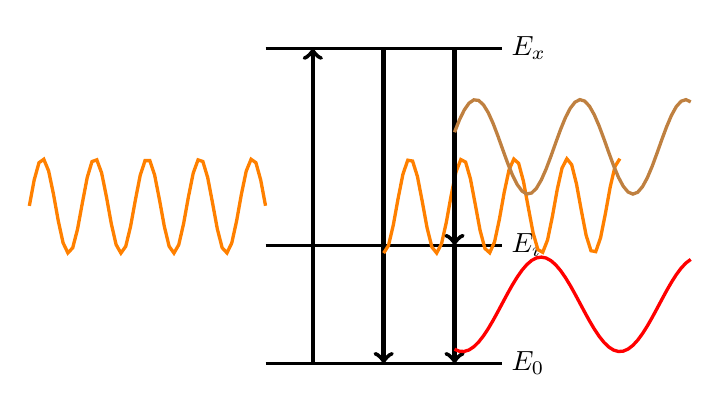
\begin{tikzpicture}
        %%% Definitions
        %% Mathematical constants
        \def \NWAVEFORMSAMPLES {50}

        %% Colors
        \def \INELASTICHIGHCOLOR {brown}
        \def \INELASTICLOWCOLOR {red}

        %% Incoming EM wave
        \def \AMPLITUDE {0.6}
        \def \WAVEFORMLENGTH {3.}
        \def \INWAVESTART {0.}
        \def \INWAVELENGTH {0.5}

        %% Outgoing EM wave
        \def \OUTWAVELENGTHHIGH {1.0}
        \def \OUTWAVELENGTHLOW {1.5}

        %% States
        \def \GROUNDSTATEY {-2.}
        \def \INTERMEDIATESTATEY {-0.5}
        \def \EXCITEDSTATEY {2.}
        \def \STATEXSTART {3.}
        \def \STATEX {3.}

        %% Transitions
        \def \EXCITATIONX {\STATEXSTART+0.2*\STATEX}
        \def \ELASTICX {\STATEXSTART+0.5*\STATEX}
        \def \INELASTICX {\STATEXSTART+0.8*\STATEX}

        %%% Drawing
        %% Incoming EM wave
        \draw [very thick, \ORANGE, domain=\INWAVESTART:\INWAVESTART+\WAVEFORMLENGTH, samples=\NWAVEFORMSAMPLES] plot (\x, {\AMPLITUDE*sin(\WAVEFORMLENGTH/\INWAVELENGTH*2*pi/4*\x r)});

        %% States
        % Ground state
        \draw[very thick, black] (\STATEXSTART, \GROUNDSTATEY) -- (\STATEXSTART+\STATEX, \GROUNDSTATEY);
        \draw (\STATEXSTART + \STATEX, \GROUNDSTATEY) node[anchor=west] {$E_0$};

        % Intermediate state
        \draw[very thick, black] (\STATEXSTART, \INTERMEDIATESTATEY) -- (\STATEXSTART+\STATEX, \INTERMEDIATESTATEY);
        \draw (\STATEXSTART + \STATEX, \INTERMEDIATESTATEY) node[anchor=west] {$E_i$};

        % Excited state
        \draw[very thick, black] (\STATEXSTART, \EXCITEDSTATEY) -- (\STATEXSTART+\STATEX, \EXCITEDSTATEY);
        \draw (\STATEXSTART + \STATEX, \EXCITEDSTATEY) node[anchor=west] {$E_x$};

        %% Transitions
        % Excitation
        \draw[->, ultra thick, black] (\EXCITATIONX, \GROUNDSTATEY) -- (\EXCITATIONX, \EXCITEDSTATEY);

        % Direct ground-state decay
        \visible<2->{
            \draw[->, ultra thick, black] (\ELASTICX, \EXCITEDSTATEY) -- (\ELASTICX, \GROUNDSTATEY);

            \draw [very thick, \ORANGE, domain=\ELASTICX:\ELASTICX+\WAVEFORMLENGTH, samples=\NWAVEFORMSAMPLES] plot (\x, {\AMPLITUDE*sin(\WAVEFORMLENGTH/\INWAVELENGTH*2*pi/4*\x r)});
        }

        % Decay via intermediate states
        \visible<3>{
            \draw[->, ultra thick, black] (\INELASTICX, \EXCITEDSTATEY) -- (\INELASTICX, \INTERMEDIATESTATEY);

            \draw [very thick, \INELASTICHIGHCOLOR, domain=\INELASTICX:\INELASTICX+\WAVEFORMLENGTH, samples=\NWAVEFORMSAMPLES] plot (\x, {\AMPLITUDE*sin(\WAVEFORMLENGTH/\OUTWAVELENGTHHIGH*2*pi/4*\x r) + \INTERMEDIATESTATEY + 0.5*(\EXCITEDSTATEY-\INTERMEDIATESTATEY)});

            \draw[->, ultra thick, black] (\INELASTICX, \INTERMEDIATESTATEY) -- (\INELASTICX, \GROUNDSTATEY);

            \draw [very thick, \INELASTICLOWCOLOR, domain=\INELASTICX:\INELASTICX+\WAVEFORMLENGTH, samples=\NWAVEFORMSAMPLES] plot (\x, {\AMPLITUDE*sin(\WAVEFORMLENGTH/\OUTWAVELENGTHLOW*2*pi/4*\x r) + \GROUNDSTATEY + 0.5*(\INTERMEDIATESTATEY-\GROUNDSTATEY)});
        }
    \end{tikzpicture}
\end{textblock}
\end{frame}

\subsection{Resonance Fluorescence in Atoms and Nuclei}

\begin{frame}
    \frametitle{Resonance Fluorescence in Atoms}
        % This file is part of nrf_seminar.

    % nrf_seminar is free software: you can redistribute it and/or modify
    % it under the terms of the GNU General Public License as published by
    % the Free Software Foundation, either version 3 of the License, or
    % (at your option) any later version.

    % nrf_seminar is distributed in the hope that it will be useful,
    % but WITHOUT ANY WARRANTY; without even the implied warranty of
    % MERCHANTABILITY or FITNESS FOR A PARTICULAR PURPOSE.  See the
    % GNU General Public License for more details.

    % You should have received a copy of the GNU General Public License
    % along with nrf_seminar.  If not, see <https://www.gnu.org/licenses/>.

\begin{textblock}{15.}(0., -4.)
    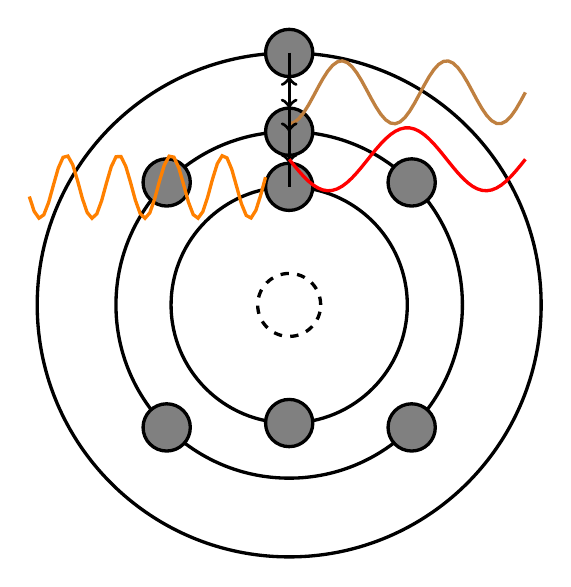
\begin{tikzpicture}
        %%% Definitions
        %% Mathematical constants
        \def \INVERSESQRTTWO {0.7071067811865475}
        \def \NWAVEFORMSAMPLES {50}

        %% Colors
        \def \INELASTICHIGHCOLOR {brown}
        \def \INELASTICLOWCOLOR {red}

        %% Incoming EM wave
        \def \AMPLITUDE {0.4}
        \def \WAVEFORMLENGTH {3.}
        \def \INWAVESTART {0.}
        \def \INWAVELENGTH {0.5}

        %% Outgoing EM wave
        \def \OUTWAVELENGTHHIGH {1.0}
        \def \OUTWAVELENGTHLOW {1.5}

        %% Atom
        \def \ELECTRONRADIUS {0.3}
        \def \ELECTRONCOLOR {gray}

        \def \ORBITALINRADIUS {1.5}
        \def \ORBITALMIDRADIUS {2.2}
        \def \ORBITALOUTRADIUS {3.2}

        \def \ATOMX {5.}
        \coordinate (ATOMPOSITION) at (\ATOMX, 0.);

        %% Nucleus
        \def \NUCLEUSRADIUS {0.4}

        %%% Drawing
        %% Atom
        % Nucleus
        \draw [very thick, black, dashed] (ATOMPOSITION) circle [radius = \NUCLEUSRADIUS];

        % Orbitals
        \draw [very thick, black] (ATOMPOSITION) circle [radius = \ORBITALINRADIUS];
        \draw [very thick, black] (ATOMPOSITION) circle [radius = \ORBITALMIDRADIUS];
        \draw [very thick, black] (ATOMPOSITION) circle [radius = \ORBITALOUTRADIUS];

        % Electrons
        % Inner electrons
        \visible<1-2,5->{
            \draw [very thick, black, fill=\ELECTRONCOLOR] ($ (ATOMPOSITION) + \ORBITALINRADIUS*(0,1)$) circle [radius = \ELECTRONRADIUS];
        }
        \visible<3>{
            \draw [very thick, black, fill=\ELECTRONCOLOR] ($ (ATOMPOSITION) + \ORBITALOUTRADIUS*(0,1)$) circle [radius = \ELECTRONRADIUS];
        }
        \visible<4>{
            \draw [very thick, black, fill=\ELECTRONCOLOR] ($ (ATOMPOSITION) + \ORBITALMIDRADIUS*(0,1)$) circle [radius = \ELECTRONRADIUS];
        }
        \draw [very thick, black, fill=\ELECTRONCOLOR] ($ (ATOMPOSITION) + \ORBITALINRADIUS*(0,-1)$) circle [radius = \ELECTRONRADIUS];

        % Outer electrons
        \draw [very thick, black, fill=\ELECTRONCOLOR] ($ (ATOMPOSITION) + \INVERSESQRTTWO*\ORBITALMIDRADIUS*(1,1)$) circle [radius = \ELECTRONRADIUS];
        \draw [very thick, black, fill=\ELECTRONCOLOR] ($ (ATOMPOSITION) + \INVERSESQRTTWO*\ORBITALMIDRADIUS*(1,-1)$) circle [radius = \ELECTRONRADIUS];
        \draw [very thick, black, fill=\ELECTRONCOLOR] ($ (ATOMPOSITION) + \INVERSESQRTTWO*\ORBITALMIDRADIUS*(-1,1)$) circle [radius = \ELECTRONRADIUS];
        \draw [very thick, black, fill=\ELECTRONCOLOR] ($ (ATOMPOSITION) + \INVERSESQRTTWO*\ORBITALMIDRADIUS*(-1,-1)$) circle [radius = \ELECTRONRADIUS];

        %% Incoming EM wave
        \visible<2>{
            \draw [very thick, \ORANGE, domain=\ATOMX-\ELECTRONRADIUS-\WAVEFORMLENGTH:\ATOMX-\ELECTRONRADIUS, samples=\NWAVEFORMSAMPLES] plot (\x, {\AMPLITUDE*sin(\WAVEFORMLENGTH/\INWAVELENGTH*2*pi/4*\x r) + \ORBITALINRADIUS});
        }

        %% Transitions
        % Excitation
        \visible<3>{
            \draw [->, very thick, black] (\ATOMX, \ORBITALINRADIUS) -- (\ATOMX, \ORBITALOUTRADIUS-\ELECTRONRADIUS);
        }
        \visible<4>{
            \draw [->, very thick, black] (\ATOMX, \ORBITALOUTRADIUS) -- (\ATOMX, \ORBITALMIDRADIUS+\ELECTRONRADIUS);
        }
        \visible<4->{
            \draw [very thick, \INELASTICHIGHCOLOR, domain=\ATOMX:\ATOMX+\WAVEFORMLENGTH, samples=\NWAVEFORMSAMPLES] plot (\x, {\AMPLITUDE*sin(\WAVEFORMLENGTH/\OUTWAVELENGTHHIGH*2*pi/4*\x r) + \ORBITALMIDRADIUS + 0.5*(\ORBITALOUTRADIUS-\ORBITALMIDRADIUS)});
        }
        \visible<5->{
            \draw [->, very thick, black] (\ATOMX, \ORBITALOUTRADIUS) -- (\ATOMX, \ORBITALMIDRADIUS);
            \draw [->, very thick, black] (\ATOMX, \ORBITALMIDRADIUS) -- (\ATOMX, \ORBITALINRADIUS+\ELECTRONRADIUS);
            \draw [very thick, \INELASTICLOWCOLOR, domain=\ATOMX:\ATOMX+\WAVEFORMLENGTH, samples=\NWAVEFORMSAMPLES] plot (\x, {\AMPLITUDE*sin(\WAVEFORMLENGTH/\OUTWAVELENGTHLOW*2*pi/4*\x r) + \ORBITALINRADIUS + 0.5*(\ORBITALMIDRADIUS-\ORBITALINRADIUS)});
        }
    \end{tikzpicture}
\end{textblock}

\begin{textblock}{5.}(8., -6.)
    \begin{center}
        \begin{tabular}{ll}
        & Atom  \\
        \hline
        Res. Energy & $\unit[10^{0}]{eV}$ \\
        Res. Width & $> \unit[10^{-7}]{eV}$ \\
        System mass $\times c^2$ & $\unit[10^{9}]{eV}$ \\
        \end{tabular}
    \end{center}
\end{textblock}

\begin{textblock}{7.}(8.5, -1.5)
    \begin{itemize}
    \visible<2->{
        \item \textbf{Photon source}: \\ 'conventional' light sources, \textbf{laser}
    }
    \visible<6>{
        \item \textbf{Photon spectroscopy}: \\
        prisms, diffraction grids
    }
    \end{itemize}
\end{textblock}

\begin{textblock}{6.}(8.5, 3.2)
    \visible<6>{
        \includegraphics[width=\textwidth]{figures/prism.jpg}
    }
\end{textblock}
\end{frame}

\begin{frame}
    \frametitle{Resonance Fluorescence in Nuclei}
    \begin{textblock}{15.}(0., -5.)
        \begin{itemize}
            \item How to achieve resonance fluorescence
            \item Recoil problem
            \item Solution of the recoil problem
            \item Artificial photon sources
        \end{itemize}
    \end{textblock}
\end{frame}

\section{Basics}

\subsection{Typical Dimensions}

\begin{frame}
    \frametitle{Nuclear Resonances}
    \begin{textblock}{15.}(0., -5.)
        \begin{itemize}
            \item Typical widths, energies
            \item Level density
        \end{itemize}
    \end{textblock}
\end{frame}

\begin{frame}
    \frametitle{Doppler Broadening}
    \begin{textblock}{15.}(0., -5.)
        \begin{itemize}
            \item Typical widths, energies
            \item Level density
            \item The special case of $^{229}$Th
        \end{itemize}
    \end{textblock}
\end{frame}

\subsection{Experiments}

\begin{frame}
    \frametitle{Why Absorption Spectroscopy is not Possible}
    \begin{textblock}{15.}(0., -5.)
        \begin{itemize}
            \item Analogy with normal vision
            \item Schematic spectrum, convolve with realistic resolution
        \end{itemize}
    \end{textblock}
\end{frame}

\begin{frame}
    \frametitle{Schematic experiment}
    \begin{textblock}{15.}(0., -5.)
        \begin{itemize}
            \item Typical setup
            \item Typical spectra
        \end{itemize}
    \end{textblock}
\end{frame}

\subsection{Photon Sources}

\begin{frame}
    \frametitle{Photon Sources}
    \begin{textblock}{15.}(0., -5.)
        \begin{itemize}
            \item Bremsstrahlung vs. Quasi-Monochromatic (Comp)
            \item Typical spectra
        \end{itemize}
    \end{textblock}
\end{frame}

\section{Applications}

\subsection{Fundamental Research}

\begin{frame}
    \frametitle{R-Process Nucleosynthesis}
    \begin{textblock}{15.}(0., -5.)
        \begin{itemize}
            \item Photodisintegration versus neutron capture
            \item Example: Pygmy Dipole Resonance
        \end{itemize}
    \end{textblock}    
\end{frame}

\subsection{Technical Applications}

\begin{frame}
    \frametitle{Isotope-selective Scanning}
\end{frame}

\end{document}